% small.tex
\documentclass{beamer}
\usepackage{amsmath,amssymb,amsthm,color}
\usepackage{movie15}
\usetheme{Madrid}

%\usepackage[pdftex]{graphicx}
%\DeclareGraphicsExtensions{.pdf,.mps,.png,.jpg}
\usepackage{subfig}
\usepackage{algorithm,algpseudocode}
\newcommand{\R}{\mathbb{R}}
\newcommand{\M}{\mathbb{M}}
\newcommand{\C}{\mathbb{C}}
\newcommand{\T}{\mathbb{T}}
\newcommand{\Sph}{\mathbb{S}}

\newcommand{\delr}{\dfrac{r}{\delta}}
\newcommand{\lp}{\left(}
\newcommand{\rp}{\right)}

\newcommand{\ep}{\varepsilon}
\newcommand{\epz}{\ep\longrightarrow 0}
\newcommand{\vect}[1]{\mathbf{#1}}
\newcommand{\vc}{\vect{c}}
\newcommand{\vf}{\vect{f}}
\newcommand{\vg}{\vect{g}}
\newcommand{\vx}{\vect{x}}
\newcommand{\vy}{\vect{y}}
\newcommand{\vxi}{\boldsymbol{\xi}}
\newcommand{\vP}{\vect{P}}
\newcommand{\vp}{\vect{p}}
\newcommand{\vH}{\vect{H}}
\newcommand{\vI}{\vect{I}}
\newcommand{\vT}{\vect{T}}
\newcommand{\vL}{\vect{L}}
\newcommand{\vn}{\vect{n}}
\newcommand{\vu}{\vect{u}}
\newcommand{\bfe}{\vect{e}}
\newcommand{\coef}{c}
\newcommand{\uu}{u_X}
\newcommand{\dt}{\Delta t}

\newcommand{\lam}{\lambda}
%\newcommand{\laps}{\Delta_{\mathcal{S}}}
%\newcommand{\Mlap}{\Delta_{\mathcal{S}}}
%\newcommand{\Mgrad}{\nabla_{\mathcal{S}}}
\newcommand{\laps}{\Delta_{\M}}
\newcommand{\Mlap}{\Delta_{\M}}
\newcommand{\Mgrad}{\nabla_{\M}}
\newcommand{\grad}{\nabla}
\newcommand{\MEgrad}{\vP\nabla}
\newcommand{\Mdiv}{\Mgrad\cdot}
\newcommand{\pder}[1]{\dfrac{\partial}{\partial#1}}
\newcommand{\pgradx}{\mathcal{G}^{x}}
\newcommand{\pgrady}{\mathcal{G}^{y}}
\newcommand{\pgradz}{\mathcal{G}^{z}}

\newcommand{\comment}[1]{{\color{red}{#1}}}

%Kevin's commands

\newcommand{\supp}{\operatorname{supp}}
\newcommand{\diag}{\mathop{\mathrm{diag}}}
\newcommand{\plotwidth}{0.4}
\newcommand{\conwidth}{0.45}
\newcommand{\diffOp}{\mathcal{L}}
\newcommand{\slfrac}[2]{\left.#1\middle/#2\right.}
\DeclareMathOperator{\sech}{sech}
\newcommand{\f}{\underline{f}}
\newcommand{\vcoefs}{\underline{c}}
\newcommand{\x}{\underline{x}}
\newcommand{\y}{\underline{y}}
\newcommand{\z}{\underline{z}}

\DeclareMathOperator*{\osc}{osc}

% items enclosed in square brackets are optional; explanation below
\title[Optimal Domain Splitting]{A 2D partition of unity adaptive refinement Chebyshev polynomial method}
\author[K. Aiton]{Kevin Aiton}
\institute[UD]{
  Department of Mathematics\\
University of Delaware\\
}
\date[October 2016]{October 30, 2017}


\begin{document}


%%%%%%%%%%%%%%%%%%%%%%%%%%%%%%%%%%%%%%%%%%%%%%%%%%%%%
%
% TITLE PAGE
%
%%%%%%%%%%%%%%%%%%%%%%%%%%%%%%%%%%%%%%%%%%%%%%%%%%%%%
\begin{frame}[plain]
  \titlepage
\end{frame}

%%%%%%%%%%%%%%%%%%%%%%%%%%%%%%%%%%%%%%%%%%%%%%%%%%%%%
%
% OUTLINE OF PRESENTATION
%
%%%%%%%%%%%%%%%%%%%%%%%%%%%%%%%%%%%%%%%%%%%%%%%%%%%%%

\begin{frame}[plain]{Outline of Presentation}

\begin{itemize}
	\item Overview of Chebyshev interpolant convergence theory
	\item Refinement of 2D Chebyshev polynomials
	\item Future work
\end{itemize}
\end{frame}

%%%%%%%%%%%%%%%%%%%%%%%%%%%%%%%%%%%%%%%%%%%%%%%%%%%%%
%
% Overview of Chebyshev polynomial convergence %theory
%
%%%%%%%%%%%%%%%%%%%%%%%%%%%%%%%%%%%%%%%%%%%%%%%%%%%%%
\begin{frame}{Overview of Chebyshev polynomial convergence theory}
We can use Chebyshev polynomials to construct approximating functions.
\begin{itemize}
\item \text{\bf Chebfun} uses polynomial interpolants based on the Chebyshev points $$x_j = \cos(j\pi/n)$$	
\item Chebyshev interpolants allow for fast and accurate algorithms for interpolation, differentiation, root finding, etc.
\end{itemize}


\end{frame}

\begin{frame}{Overview of Chebyshev polynomial convergence theory}

Chebyshev points are special because they allow for \textbf{spectral} convergence.

\begin{itemize}
\item Key idea: If $f(x) = \sum_{i=0}^{\infty} a_i T_i(x)$, then for the interpolant $p_n(x)$ $$ \|f(x) - p_n \|_{\infty} \leq 2 \sum_{i=n+1}^{\infty} |a_i|.$$
\item Chebfun uses the coefficients {\tt standardChop} to determine the degree of $p_n(x)$ for a given tolerance.
\end{itemize}

\end{frame}

\begin{frame}{Chopping a Chebfun polynomial}
\begin{center}
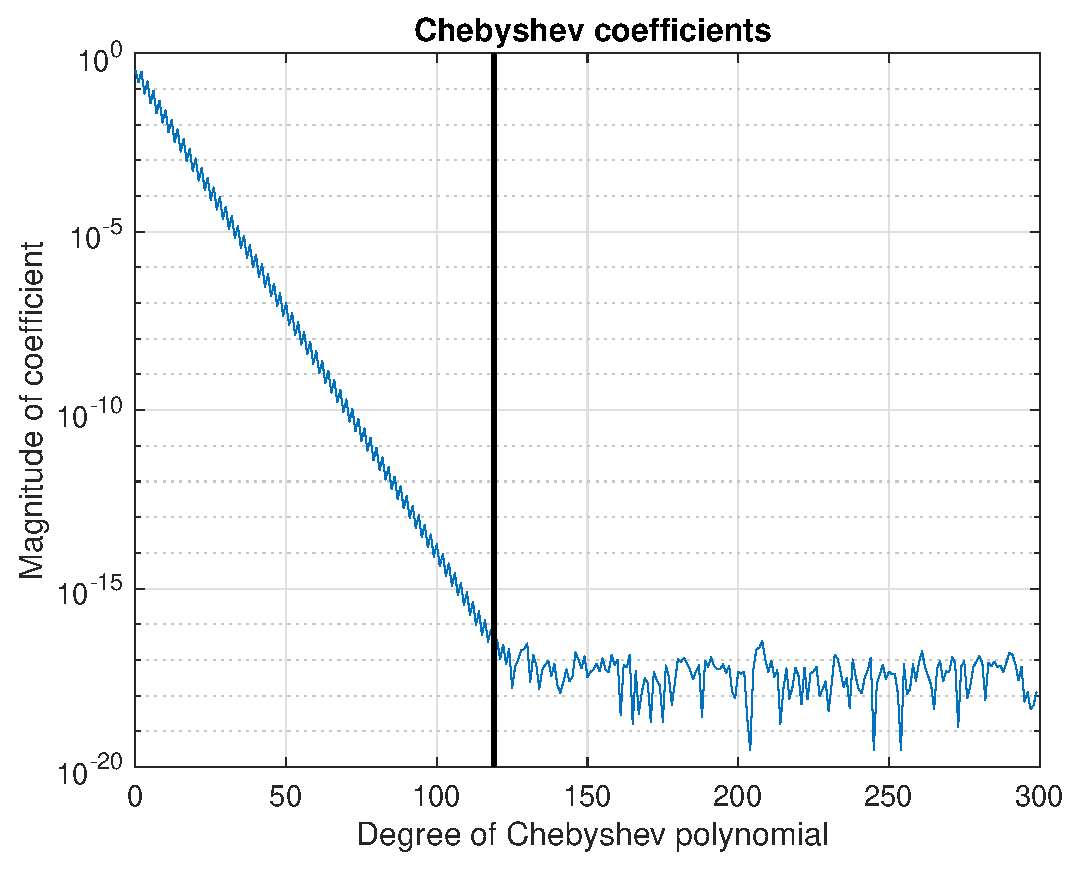
\includegraphics[scale = 0.4]{Cheb15.eps}
\end{center}

\begin{center}
\begin{itemize}
\item \begin{center} Coefficients for $f(x)=\exp(x)/(1+10 x^2)$. \end{center}
\item \begin{center} with tol=$10^{-15}$, $n=119$ \end{center}
\item \begin{center} $\| f(x)-p_n(x) \|_{\infty}$ = 1.0e-14 \end{center}
\end{itemize} 
\end{center}
\end{frame}

\begin{frame}{Chopping a Chebfun polynomial}
\begin{center}
\includegraphics[scale = 0.4]{Cheb8.eps}
\end{center}

\begin{center}
\begin{itemize}
\item \begin{center} Coefficients for $f(x)=\exp(x)/(1+10 x^2)$. \end{center}
\item \begin{center} with tol=$10^{-8}$, $n=71$ \end{center}
\item \begin{center} $\| f(x)-p_n(x) \|_{\infty}$ = 1.1e-8 \end{center}
\end{itemize}
\end{center}
\end{frame}

\begin{frame}{Refinement for 2D tensor product polynomials}
\begin{itemize}
\item We seek to do something similar for $f(x,y)$ via a tensor product approximation $$ p(x,y) = \sum_{i=0}^{N_x} \sum_{j=0}^{N_y} T_i(x)T_j(y) a_{ij}$$
\end{itemize}

\begin{theorem} 
Let $f:[-1,1]^2 \to \R$ be Lipschitz continuous. Then for $\varepsilon>0$ there exists $N_x,N_y$ such that
$$
\|f(x,y)-p(x,y)\|_{\infty} \leq \varepsilon.
$$
 \end{theorem}

\end{frame}

\begin{frame}{Refinement for 2D tensor product polynomials}
\begin{itemize}
\item With $$
 	c_j(x) = \frac{2 \hat{\delta_j}}{\pi} \int_{-1}^{1} \frac{1}{\sqrt{1-y^2}}T_j(y)f(x,y)dy.
$$ we have for fixed $\hat{x}$
$$
f(\hat{x},y) \approx \sum_{j=0}^{N_y}T_j(y)c_j(\hat{x})
$$
and for fixed $\hat{y}$
$$
p(x,\hat{y}) = \sum_{i=0}^{N_x} \T_i(x) \frac{2 \hat{\delta_i}}{\pi} \int_{-1}^{1} \frac{1}{\sqrt{1-x^2}} \sum_{j=0}^{N_y}T_j(\hat{y})c_j(x) dx.
$$

\end{itemize}
\end{frame}


\begin{frame}[t]{Refinement for 2D tensor product polynomials}

\begin{center}
Key idea of proof: with $$p(x,y)=\sum_{i=0}^{N_x} T_i(x) \sum_{j=0}^{N_y} T_j(y)a_{ij}$$
\end{center}

\begin{columns}[t]
\begin{column}[t]{0.5\textwidth}
We can find $N_y$ such that
$$\|f(\cdot,y) -\sum_{i=0}^{N_y} c_j(\cdot)T_j(y) \| \leq \varepsilon/2$$
\end{column}
\begin{column}[t]{0.5\textwidth}
\begin{center}
We can then find $N_x$ such that
$$\|p(x,\cdot) - \sum_{i=0}^{N_y} c_j(x)T_j(\cdot)\|<\varepsilon/2,$$
\end{center}	
\end{column}

\end{columns}

\end{frame}


\begin{frame}{Refinement for 2D tensor product polynomials}
\begin{center}
We can test $\|f(\cdot,y) -\sum_{i=0}^{N_y} c_j(\cdot)T_j(y) \| \leq \varepsilon/2$ discretely by testing the series  $\{f(x_k,y)\}$ for the Chebyshev points $\{x_k\}$.
\end{center}

\begin{center}
For coefficients computed with FFT, we have,
$$ c_j(x_k) = \sum_{i=0}^{N_x}T_j(x_k)a_{ij}. $$
\end{center}

\begin{center}
We thus have
$$ |c_j(x_k)| < \sum_{i=0}^{N_x} |a_{ij}|. $$ We use {\tt StandardChop} on $\{ \sum_{i=0}^{N_x} |a_{ij}|  \}_{j=0}^{N_y}$ to test for the condition.
\end{center}

\end{frame}

\begin{frame}{Refinement for 2D tensor product polynomials}

\begin{center}
\includegraphics[scale = 0.5]{absCoeffs.eps}
\end{center}

\end{frame}

\begin{frame}{Refinement for 2D tensor product polynomials}
\begin{center}
To test for $\|p(x,\cdot) - \sum_{i=0}^{N_y} c_j(x)T_j(\cdot)\|<\varepsilon/2$, we note: $$p(x,\cdot)=\sum_{i=0}^{N_x} T_i(x) \sum_{j=0}^{N_y} T_j(\cdot)a_{ij}$$
and
$$ \left | \sum_{j=0}^{N_y} T_j(\cdot)a_{ij} \right | < \sum_{j=0}^{N_y} |a_{ij}|. $$
\end{center}

\begin{center}
We use {\tt StandardChop} on $\{ \sum_{j=0}^{N_y} |a_{ij}|  \}_{i=0}^{N_x}$ to test for the condition.
\end{center}
\end{frame}

\begin{frame}{Refinement for 2D tensor product polynomials}
\begin{center}
This gives us a discrete test for convergence:
\end{center}

\begin{center}
Run	{\tt standardChop} on $\{ \sum_{i=0}^{N_x} |a_{ij}|  \}_{j=0}^{N_y}$ and $\{ \sum_{j=0}^{N_y} |a_{ij}|  \}_{i=0}^{N_x}$.
\end{center}

\end{frame}

\begin{frame}{Partition of unity method}
\begin{center}
To refine, we cannot just increase $N_x$ and $N_y$. $N_x N_y$ gets big!
\end{center}

\begin{itemize}
\item We instead split $[-1,1] \times [-1,1]$ into overlapping squares $\{ \Omega_k \}$.
\item With approximations $s_k:\Omega_k \to \R$, we define a partition of unity $w_k:\Omega_k \to \R$ with $\sum_k w_k=1$ so we get an approximation $$s(\vect{x}) = \sum_k w_k(\vect{x})s_k(\vect{x}).$$
\end{itemize}

\end{frame}

\begin{frame}{Partition of unity method}
\begin{center}
The domains are defined by the leaves of a kd-tree, where each split is defined by splitting the square in half with a line.
\end{center}

\begin{center}
\includegraphics[scale = 0.4]{zonePlot.eps}
\end{center}
\end{frame}

\begin{frame}{Partition of unity method}
\begin{center}
For each leaf of the tree, we form the domain by 'pudging out' the rectangle.
\end{center}

\begin{center}
\includegraphics[scale = 0.4]{domainPlot.eps}
\end{center}
\end{frame}

\begin{frame}{Partition of unity method}
\begin{center}
We build an approximation by recursively splitting the tree until for every leaf $\nu_k$ we have:
\end{center}
\begin{itemize}
\item For the polynomial approximation $s_k(x,y)=\sum_{i=0}^{N_x} T_i(x) \sum_{j=0}^{N_y} T_j(y)a_{ij}$ on $\Omega_k$, both $$ \left \{ \sum_{j=0}^{N_y} |a_{ij}|  \right \}_{i=0}^{N_x}, \left \{ \sum_{i=0}^{N_x} |a_{ij}|  \right \}_{j=0}^{N_y} $$ pass the { \tt StandardChop } test.
\end{itemize}

\end{frame}

\begin{frame}{Partition of unity method}

\begin{center}
Here we adaptively build an approximation $s(x,y)$ for $f(x,y) = \arctan \lp \lp x^2+y \rp/0.01 \rp$ with tol=$10^{-12}$.
\end{center}

\begin{columns}[t]

\begin{column}{0.5\textwidth}	
\begin{center}
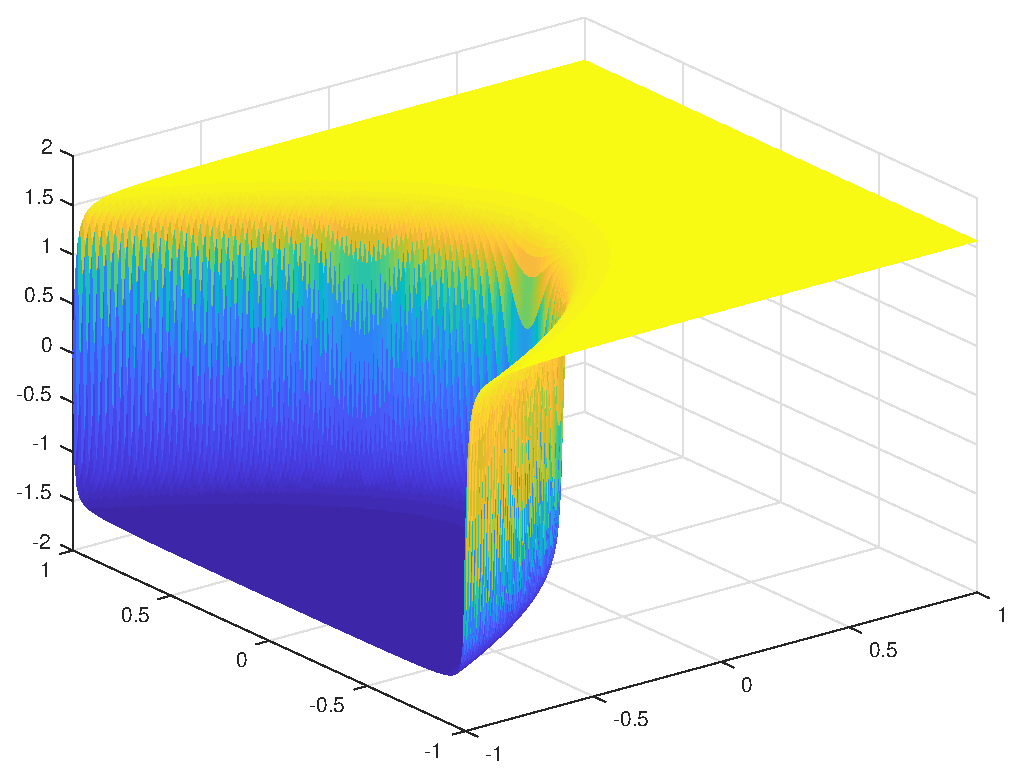
\includegraphics[scale = 0.3]{tan2Dplot.eps}	
\end{center}
\end{column}

\begin{column}{0.5\textwidth}
\begin{center}
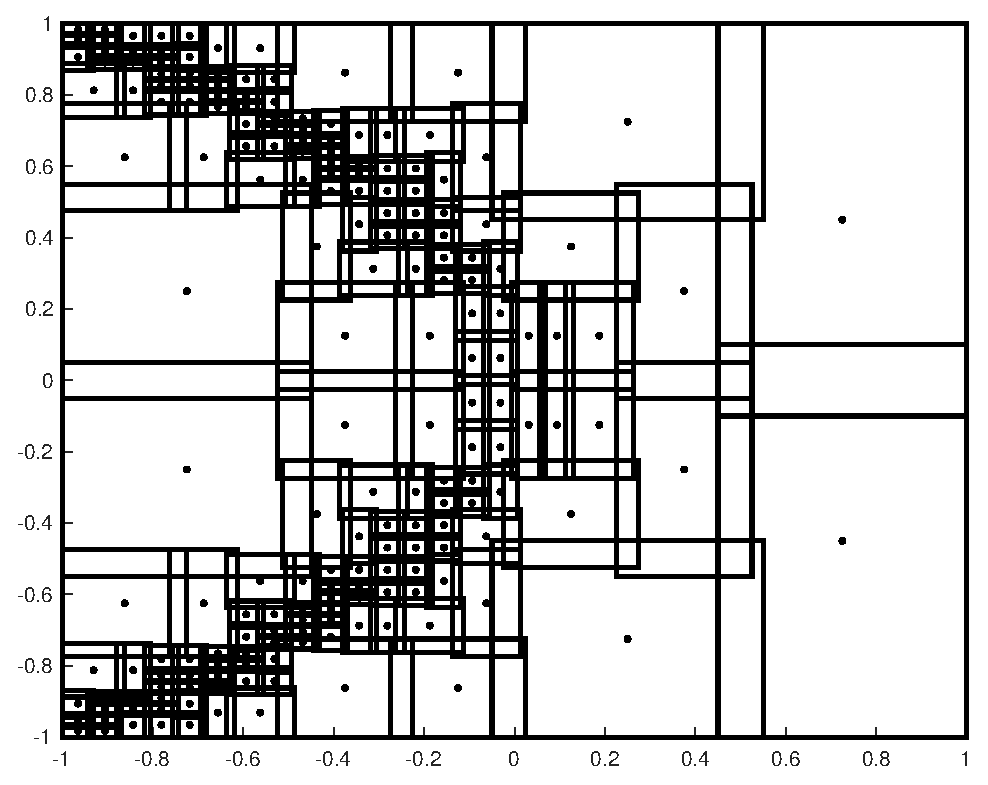
\includegraphics[scale = 0.3]{tan2Dsubdomains.eps}	
\end{center}
\end{column}

\end{columns}

\begin{center}
took 1.5 seconds to build, $\| s(x,y)-f(x,y)\|_{\infty} = 6\times10^{-14}$.	
\end{center}

\end{frame}

\begin{frame}{Further Work}
	\begin{center}
		We are currently working on an adaptive \textbf{alternating Schwarz} method for solving boundary value problems. To solve $\mathcal{L}(u)=f$ in $\Omega$, $u=g$ on $\partial G$ we:
	\end{center}
	
	\begin{center}
	for $n=1,2,\dots$ solve
	\begin{equation*}
	\begin{aligned}
	&\mathcal{L}(u_1^{n+1})=f \\
	&u_1^{n+1} = g \text{ at } \partial\Omega_1 \cap \partial\Omega \\
	&u_1^{n+1} = u_2^{n} \text{ at } \partial\Omega_1 \setminus \partial\Omega 
	\end{aligned} \quad 	\begin{aligned}
	&\mathcal{L}(u_2^{n+1})=f \\
	&u_2^{n+1} = g \text{ at } \partial\Omega_1 \cap \partial\Omega \\
	&u_2^{n+1} = u_1^{n} \text{ at } \partial\Omega_1 \setminus \partial\Omega 
	\end{aligned}
	\end{equation*}	
	\end{center}

\end{frame}

\begin{frame}{Further Work}
	\begin{center}
		We are currently working on an adaptive \textbf{alternating Schwarz} method for solving boundary value problems. We develop a scheme where:
	\end{center}
	\begin{center}
		We use the overlapping subdomains from a kd-tree.
	\end{center}

	\begin{center}
		\includegraphics[scale = 0.3]{ASdomain1.eps}
	\end{center}
\end{frame}

\begin{frame}{Further Work}
	\begin{center}
		We are currently working on an adaptive \textbf{alternating Schwarz} method for solving boundary value problems. We develop a scheme where:
	\end{center}
	\begin{center}
		For border interpolation of $\partial \Omega_k$, we interpolant $s_j(x,y)$ if $(x,y)$ is in the non overlapping square of leaf $j$.
	\end{center}

	\begin{center}
		\includegraphics[scale = 0.3]{ASdomain2.eps}
	\end{center}
\end{frame}

\begin{frame}{Further Work}
	\begin{center}
		We are currently working on an adaptive \textbf{alternating Schwarz} method for solving boundary value problems. We develop a scheme where:
	\end{center}
	\begin{center}
		After obtaining a solution, splitting the leaves using the scheme we defined before.
	\end{center}

	\begin{center}
		\includegraphics[scale = 0.3]{zonePlot2.eps}
	\end{center}
\end{frame}

\begin{frame}{Further Work}
\begin{itemize}
\item We use GMRES to solve the alternating Schwarz method.
\item We are currently developing a preconditioner that appears to keep the number of GMRES iterations constant.	
\end{itemize}

\end{frame}

\begin{frame}{Resources}
\begin{thebibliography}{9}
\bibitem{DriscollWeideman2014} 
Tobin A. Driscoll, and J.A.C. Weideman
\textit{Optimal Domain Splitting for Interpolation by Chebyshev Polynomials}. 
Siam Journal of Numerical Analysis, 2014
\bibitem{ApproxTref} 
Lloyd N. Trefethen,
\textit{Approximation Theory and Approximation Practice}. 
SIAM
\bibitem{cheb} 
\textit{Chebfun}. 
http://www.chebfun.org
\end{thebibliography}
\end{frame}

\end{document}